\documentclass[11pt,a4paper]{book}
\usepackage{pifont}
\usepackage{color}
\usepackage{graphicx}
\usepackage{subfigure}
\usepackage{fancyhdr}
\usepackage{subeqnarray}
\usepackage{ifthen}
\usepackage[hyperindex,pagebackref=true]{hyperref}
\usepackage{supertabular}
\usepackage{moreverb}
\usepackage{fancyvrb}
\usepackage{listings}
\usepackage{natbib}
\usepackage{doi}
\usepackage{longtable}
\usepackage{pdflscape}
\usepackage{psfrag}
\usepackage{makeidx}
\usepackage{palatino}
\usepackage{epsfig}
\usepackage{multirow}
\usepackage{rotating} 

%Flag for htlatex compilation to html.
\newboolean{HTLatex}
\setboolean{HTLatex}{false}
\newcommand{\ifhtml}[2]{\ifthenelse{\boolean{HTLatex}}{#1}{#2}}
\newcommand{\onlypdf}[1]{\ifthenelse{\boolean{HTLatex}}{}{#1}}
\newcommand{\onlyhtml}[1]{\ifthenelse{\boolean{HTLatex}}{#1}{}}
\newcommand{\targetlabel}[1]{\hypertarget{#1}{}\label{#1}}

\usepackage{pdftricks}
\usepackage{pstricks}
\usepackage{pst-node}
\begin{psinputs}
  \usepackage{palatino}
  \usepackage{color}
  \usepackage{pst-node}
  \usepackage{graphicx}
  \usepackage{psfrag}
  \usepackage{units}
\usepackage{xspace}
\usepackage{amsfonts,amsmath,amssymb,amsthm,amsbsy,amssymb,bm}

% Place any maths notation which is also required in figures here.

% Text abbreviations.
\newcommand{\ie}{{\em{i.e., }}}
\newcommand{\eg}{{\em{e.g., }}}
\newcommand{\cf}{{\em{cf., }}}
\newcommand{\fluidity}{Fluidity\xspace}
\newcommand{\wrt}{with respect to}
\newcommand{\lhs}{left hand side}
\newcommand{\rhs}{right hand side}
\newcommand{\fluiditysourcepath}{{\tt$\textless\textless$fluidity\_source\_path$\textgreater\textgreater$}}

% Commands definining mathematical notation.

% This is for quantities which are physically vectors.
\renewcommand{\vec}[1]{{\mbox{\boldmath$#1$}}}
% Physical rank 2 tensors
\newcommand{\tensor}[1]{\overline{\overline{#1}}}
% This is for vectors formed of the value of a quantity at each node.
\newcommand{\dvec}[1]{\underline{#1}}
% This is for matrices in the discrete system.
\newcommand{\mat}[1]{\mathrm{#1}}

\renewcommand{\div}{\nabla\cdot}
\newcommand{\grad}{\nabla}
\newcommand{\curl}{\nabla\cross}

% The domain boundary.
\newcommand{\dOmega}{{\partial\Omega}}

\DeclareMathOperator{\sgn}{sgn}
\newtheorem{thm}{Theorem}[section]
\newtheorem{lemma}[thm]{Lemma}

%\newcommand\qed{\hfill\mbox{$\Box$}}
\newcommand{\re}{{\mathrm{I}\hspace{-0.2em}\mathrm{R}}}
\newcommand{\inner}[2]{\langle#1,#2\rangle}
\renewcommand\leq{\leqslant}
\renewcommand\geq{\geqslant}
\renewcommand\le{\leqslant}
\renewcommand\ge{\geqslant}
\renewcommand\epsilon{\varepsilon}
\newcommand\eps{\varepsilon}
\renewcommand\phi{\varphi}
\newcommand{\bmF}{\vec{F}}
\newcommand{\bmphi}{\vec{\phi}}
\newcommand{\bmn}{\vec{n}}
\newcommand{\bmns}{{\textrm{\scriptsize{\boldmath $n$}}}}
\newcommand{\bmi}{\vec{i}}
\newcommand{\bmj}{\vec{j}}
\newcommand{\bmk}{\vec{k}}
\newcommand{\bmx}{\vec{x}}
\newcommand{\bmu}{\vec{u}}
\newcommand{\bmv}{\vec{v}}
\newcommand{\bmr}{\vec{r}}
\newcommand{\bma}{\vec{a}}
\newcommand{\bmg}{\vec{g}}
\newcommand{\bmU}{\vec{U}}
\newcommand{\bmI}{\vec{I}}
\newcommand{\bmq}{\vec{q}}
\newcommand{\bmT}{\vec{T}}
\newcommand{\bmM}{\vec{M}}
\newcommand{\bmtau}{\vec{\tau}}
\newcommand{\bmOmega}{\vec{\Omega}}
\bmdefine{\bmphi}{\phi}
\newcommand{\pp}{\partial}
\newcommand{\kaptens}{\tensor{\kappa}}
\newcommand{\tautens}{\tensor{\tau}}
\newcommand{\sigtens}{\tensor{\sigma}}
\newcommand{\etens}{\tensor{\dot\epsilon}}
\newcommand{\ktens}{\tensor{k}}
\newcommand{\half}{{\textstyle \frac{1}{2}}}
\newcommand{\tote}{E}
\newcommand{\inte}{e}
\newcommand{\strt}{\dot\epsilon}
\newcommand{\modu}{|\bmu|}
% discretised pressure gradient operator/matrix
\newcommand{\matC}{\mat C}
% discretised divergence operator/matrix
\newcommand{\matB}{\mat B}
% Derivatives
\renewcommand{\d}{\mathrm{d}}
\newcommand{\D}{\mathrm{D}}
\newcommand{\ddx}[2][x]{\frac{\d#2}{\d#1}}
\newcommand{\ddxx}[2][x]{\frac{\d^2#2}{\d#1^2}}
\newcommand{\ddt}[2][t]{\frac{\d#2}{\d#1}}
\newcommand{\ddtt}[2][t]{\frac{\d^2#2}{\d#1^2}}
\newcommand{\ppx}[2][x]{\frac{\partial#2}{\partial#1}}
\newcommand{\ppxx}[2][x]{\frac{\partial^2#2}{\partial#1^2}}
\newcommand{\ppt}[2][t]{\frac{\partial#2}{\partial#1}}
\newcommand{\pptt}[2][t]{\frac{\partial^2#2}{\partial#1^2}}
\newcommand{\DDx}[2][x]{\frac{\D#2}{\D#1}}
\newcommand{\DDxx}[2][x]{\frac{\D^2#2}{\D#1^2}}
\newcommand{\DDt}[2][t]{\frac{\D#2}{\D#1}}
\newcommand{\DDtt}[2][t]{\frac{\D^2#2}{\D#1^2}}
% Norms
\newcommand{\Ltwo}{\ensuremath{L_2} }
% Basis functions
\newcommand{\Qone}{\ensuremath{Q_1} }
\newcommand{\Qtwo}{\ensuremath{Q_2} }
\newcommand{\Qthree}{\ensuremath{Q_3} }
\newcommand{\QN}{\ensuremath{Q_N} }
\newcommand{\Pzero}{\ensuremath{P_0} }
\newcommand{\Pone}{\ensuremath{P_1} }
\newcommand{\Ptwo}{\ensuremath{P_2} }
\newcommand{\Pthree}{\ensuremath{P_3} }
\newcommand{\PN}{\ensuremath{P_N} }
\newcommand{\PNN}{\ensuremath{P_NP_N} }
\newcommand{\Poo}{\ensuremath{P_1P_1} }
\newcommand{\PoDG}{\ensuremath{P_{1\mathrm{DG}}} }
\newcommand{\PoDGPt}{\ensuremath{P_{1\mathrm{DG}}P_2} }
\newcommand{\Pzo}{\ensuremath{P_0P_1} }
\newcommand{\Poz}{\ensuremath{P_1P_0} }
\newcommand{\PzoCV}{\ensuremath{P_0P_{1\mathrm{CV}}} }

\newcommand{\metric}{\tensor{M}}
\newcommand{\configureflag}[1]{\texttt{#1}}

% Nonlinear relaxation parameter.
\newcommand{\thetanl}{\theta_{\mathrm{nl}}}
% Implicitness parameters.
\newcommand{\thetac}{\theta_c}
\newcommand{\thetau}{\theta_{\vec{u}}}

% Notation used in timestepping.
\newcommand{\ustar}{\dvec{u}_*}
\newcommand{\unew}{\dvec{\tilde u}^{n+1}}
\newcommand{\uold}{\dvec{u}^{n}}
\newcommand{\urelax}{\vec{u}^{n+\thetanl}}
\newcommand{\pstar}{\dvec{p}_*}
\newcommand{\pnew}{\dvec{\tilde p}^{n+1}}

\newcommand{\cnew}{\dvec{\tilde c}^{n+1}}
\newcommand{\ctheta}{\dvec{c}^{n+\thetac}}
\newcommand{\cold}{\dvec{c}^{n}}
\newcommand{\cstar}{\dvec{c}_*}

\newcommand{\rhonew}{\dvec{\tilde \rho}^{n+1}}
\newcommand{\rhoold}{\dvec{\rho}^{n}}
\newcommand{\rhorelax}{\rho^{n+\thetanl}}


% Units
\newcommand{\m}[1][]{\unit[#1]{m}}
\newcommand{\km}[1][]{\unit[#1]{km}}
\newcommand{\s}[1][]{\unit[#1]{s}}
\newcommand{\invs}[1][]{\unit[#1]{s}\ensuremath{^{-1}}}
\newcommand{\ms}[1][]{\unit[#1]{m\ensuremath{\,}s\ensuremath{^{-1}}}}
\newcommand{\mss}[1][]{\unit[#1]{m\ensuremath{\,}s\ensuremath{^{-2}}}}
\newcommand{\K}[1][]{\unit[#1]{K}}
\newcommand{\PSU}[1][]{\unit[#1]{PSU}}
\newcommand{\Pa}[1][]{\unit[#1]{Pa}}
\newcommand{\kg}[1][]{\unit[#1]{kg}}
\newcommand{\rads}[1][]{\unit[#1]{rad\ensuremath{\,}s\ensuremath{^{-1}}}}
\newcommand{\kgmm}[1][]{\unit[#1]{kg\ensuremath{\,}m\ensuremath{^{-2}}}}
\newcommand{\kgmmm}[1][]{\unit[#1]{kg\ensuremath{\,}m\ensuremath{^{-3}}}}
\newcommand{\Nmm}[1][]{\unit[#1]{N\ensuremath{\,}m\ensuremath{^{-2}}}}

% Dimensionless numbers
\newcommand{\dimensionless}[1]{\mathrm{#1}}
\renewcommand{\Re}{\dimensionless{Re}}
\newcommand{\Ro}{\dimensionless{Ro}}
\newcommand{\Fr}{\dimensionless{Fr}}
\newcommand{\Bu}{\dimensionless{Bu}}
\newcommand{\Ri}{\dimensionless{Ri}}
\renewcommand{\Pr}{\dimensionless{Pr}}
\newcommand{\Pe}{\dimensionless{Pe}}
\newcommand{\Ek}{\dimensionless{Ek}}
\newcommand{\Gr}{\dimensionless{Gr}}
\newcommand{\Ra}{\dimensionless{Ra}}


\end{psinputs}

\newcommand{\note}[1]{\textbf{Note: #1}}

\usepackage{units}
\usepackage{xspace}
\usepackage{amsfonts,amsmath,amssymb,amsthm,amsbsy,amssymb,bm}

% Place any maths notation which is also required in figures here.

% Text abbreviations.
\newcommand{\ie}{{\em{i.e., }}}
\newcommand{\eg}{{\em{e.g., }}}
\newcommand{\cf}{{\em{cf., }}}
\newcommand{\fluidity}{Fluidity\xspace}
\newcommand{\wrt}{with respect to}
\newcommand{\lhs}{left hand side}
\newcommand{\rhs}{right hand side}
\newcommand{\fluiditysourcepath}{{\tt$\textless\textless$fluidity\_source\_path$\textgreater\textgreater$}}

% Commands definining mathematical notation.

% This is for quantities which are physically vectors.
\renewcommand{\vec}[1]{{\mbox{\boldmath$#1$}}}
% Physical rank 2 tensors
\newcommand{\tensor}[1]{\overline{\overline{#1}}}
% This is for vectors formed of the value of a quantity at each node.
\newcommand{\dvec}[1]{\underline{#1}}
% This is for matrices in the discrete system.
\newcommand{\mat}[1]{\mathrm{#1}}

\renewcommand{\div}{\nabla\cdot}
\newcommand{\grad}{\nabla}
\newcommand{\curl}{\nabla\cross}

% The domain boundary.
\newcommand{\dOmega}{{\partial\Omega}}

\DeclareMathOperator{\sgn}{sgn}
\newtheorem{thm}{Theorem}[section]
\newtheorem{lemma}[thm]{Lemma}

%\newcommand\qed{\hfill\mbox{$\Box$}}
\newcommand{\re}{{\mathrm{I}\hspace{-0.2em}\mathrm{R}}}
\newcommand{\inner}[2]{\langle#1,#2\rangle}
\renewcommand\leq{\leqslant}
\renewcommand\geq{\geqslant}
\renewcommand\le{\leqslant}
\renewcommand\ge{\geqslant}
\renewcommand\epsilon{\varepsilon}
\newcommand\eps{\varepsilon}
\renewcommand\phi{\varphi}
\newcommand{\bmF}{\vec{F}}
\newcommand{\bmphi}{\vec{\phi}}
\newcommand{\bmn}{\vec{n}}
\newcommand{\bmns}{{\textrm{\scriptsize{\boldmath $n$}}}}
\newcommand{\bmi}{\vec{i}}
\newcommand{\bmj}{\vec{j}}
\newcommand{\bmk}{\vec{k}}
\newcommand{\bmx}{\vec{x}}
\newcommand{\bmu}{\vec{u}}
\newcommand{\bmv}{\vec{v}}
\newcommand{\bmr}{\vec{r}}
\newcommand{\bma}{\vec{a}}
\newcommand{\bmg}{\vec{g}}
\newcommand{\bmU}{\vec{U}}
\newcommand{\bmI}{\vec{I}}
\newcommand{\bmq}{\vec{q}}
\newcommand{\bmT}{\vec{T}}
\newcommand{\bmM}{\vec{M}}
\newcommand{\bmtau}{\vec{\tau}}
\newcommand{\bmOmega}{\vec{\Omega}}
\bmdefine{\bmphi}{\phi}
\newcommand{\pp}{\partial}
\newcommand{\kaptens}{\tensor{\kappa}}
\newcommand{\tautens}{\tensor{\tau}}
\newcommand{\sigtens}{\tensor{\sigma}}
\newcommand{\etens}{\tensor{\dot\epsilon}}
\newcommand{\ktens}{\tensor{k}}
\newcommand{\half}{{\textstyle \frac{1}{2}}}
\newcommand{\tote}{E}
\newcommand{\inte}{e}
\newcommand{\strt}{\dot\epsilon}
\newcommand{\modu}{|\bmu|}
% discretised pressure gradient operator/matrix
\newcommand{\matC}{\mat C}
% discretised divergence operator/matrix
\newcommand{\matB}{\mat B}
% Derivatives
\renewcommand{\d}{\mathrm{d}}
\newcommand{\D}{\mathrm{D}}
\newcommand{\ddx}[2][x]{\frac{\d#2}{\d#1}}
\newcommand{\ddxx}[2][x]{\frac{\d^2#2}{\d#1^2}}
\newcommand{\ddt}[2][t]{\frac{\d#2}{\d#1}}
\newcommand{\ddtt}[2][t]{\frac{\d^2#2}{\d#1^2}}
\newcommand{\ppx}[2][x]{\frac{\partial#2}{\partial#1}}
\newcommand{\ppxx}[2][x]{\frac{\partial^2#2}{\partial#1^2}}
\newcommand{\ppt}[2][t]{\frac{\partial#2}{\partial#1}}
\newcommand{\pptt}[2][t]{\frac{\partial^2#2}{\partial#1^2}}
\newcommand{\DDx}[2][x]{\frac{\D#2}{\D#1}}
\newcommand{\DDxx}[2][x]{\frac{\D^2#2}{\D#1^2}}
\newcommand{\DDt}[2][t]{\frac{\D#2}{\D#1}}
\newcommand{\DDtt}[2][t]{\frac{\D^2#2}{\D#1^2}}
% Norms
\newcommand{\Ltwo}{\ensuremath{L_2} }
% Basis functions
\newcommand{\Qone}{\ensuremath{Q_1} }
\newcommand{\Qtwo}{\ensuremath{Q_2} }
\newcommand{\Qthree}{\ensuremath{Q_3} }
\newcommand{\QN}{\ensuremath{Q_N} }
\newcommand{\Pzero}{\ensuremath{P_0} }
\newcommand{\Pone}{\ensuremath{P_1} }
\newcommand{\Ptwo}{\ensuremath{P_2} }
\newcommand{\Pthree}{\ensuremath{P_3} }
\newcommand{\PN}{\ensuremath{P_N} }
\newcommand{\PNN}{\ensuremath{P_NP_N} }
\newcommand{\Poo}{\ensuremath{P_1P_1} }
\newcommand{\PoDG}{\ensuremath{P_{1\mathrm{DG}}} }
\newcommand{\PoDGPt}{\ensuremath{P_{1\mathrm{DG}}P_2} }
\newcommand{\Pzo}{\ensuremath{P_0P_1} }
\newcommand{\Poz}{\ensuremath{P_1P_0} }
\newcommand{\PzoCV}{\ensuremath{P_0P_{1\mathrm{CV}}} }

\newcommand{\metric}{\tensor{M}}
\newcommand{\configureflag}[1]{\texttt{#1}}

% Nonlinear relaxation parameter.
\newcommand{\thetanl}{\theta_{\mathrm{nl}}}
% Implicitness parameters.
\newcommand{\thetac}{\theta_c}
\newcommand{\thetau}{\theta_{\vec{u}}}

% Notation used in timestepping.
\newcommand{\ustar}{\dvec{u}_*}
\newcommand{\unew}{\dvec{\tilde u}^{n+1}}
\newcommand{\uold}{\dvec{u}^{n}}
\newcommand{\urelax}{\vec{u}^{n+\thetanl}}
\newcommand{\pstar}{\dvec{p}_*}
\newcommand{\pnew}{\dvec{\tilde p}^{n+1}}

\newcommand{\cnew}{\dvec{\tilde c}^{n+1}}
\newcommand{\ctheta}{\dvec{c}^{n+\thetac}}
\newcommand{\cold}{\dvec{c}^{n}}
\newcommand{\cstar}{\dvec{c}_*}

\newcommand{\rhonew}{\dvec{\tilde \rho}^{n+1}}
\newcommand{\rhoold}{\dvec{\rho}^{n}}
\newcommand{\rhorelax}{\rho^{n+\thetanl}}


% Units
\newcommand{\m}[1][]{\unit[#1]{m}}
\newcommand{\km}[1][]{\unit[#1]{km}}
\newcommand{\s}[1][]{\unit[#1]{s}}
\newcommand{\invs}[1][]{\unit[#1]{s}\ensuremath{^{-1}}}
\newcommand{\ms}[1][]{\unit[#1]{m\ensuremath{\,}s\ensuremath{^{-1}}}}
\newcommand{\mss}[1][]{\unit[#1]{m\ensuremath{\,}s\ensuremath{^{-2}}}}
\newcommand{\K}[1][]{\unit[#1]{K}}
\newcommand{\PSU}[1][]{\unit[#1]{PSU}}
\newcommand{\Pa}[1][]{\unit[#1]{Pa}}
\newcommand{\kg}[1][]{\unit[#1]{kg}}
\newcommand{\rads}[1][]{\unit[#1]{rad\ensuremath{\,}s\ensuremath{^{-1}}}}
\newcommand{\kgmm}[1][]{\unit[#1]{kg\ensuremath{\,}m\ensuremath{^{-2}}}}
\newcommand{\kgmmm}[1][]{\unit[#1]{kg\ensuremath{\,}m\ensuremath{^{-3}}}}
\newcommand{\Nmm}[1][]{\unit[#1]{N\ensuremath{\,}m\ensuremath{^{-2}}}}

% Dimensionless numbers
\newcommand{\dimensionless}[1]{\mathrm{#1}}
\renewcommand{\Re}{\dimensionless{Re}}
\newcommand{\Ro}{\dimensionless{Ro}}
\newcommand{\Fr}{\dimensionless{Fr}}
\newcommand{\Bu}{\dimensionless{Bu}}
\newcommand{\Ri}{\dimensionless{Ri}}
\renewcommand{\Pr}{\dimensionless{Pr}}
\newcommand{\Pe}{\dimensionless{Pe}}
\newcommand{\Ek}{\dimensionless{Ek}}
\newcommand{\Gr}{\dimensionless{Gr}}
\newcommand{\Ra}{\dimensionless{Ra}}



\makeindex
% Command to enable the labelling of the primary reference. 
% To do this use \index{term|primary}
\newcommand{\primary}[1]{\textbf{\hyperpage{#1}}}

% Cause numbering of subsubsections. 
\setcounter{secnumdepth}{3}

\definecolor{DarkBlue}{rgb}{0.00,0.00,0.55}
\hypersetup{
    linkcolor   = DarkBlue,
    anchorcolor = DarkBlue,
    citecolor   = DarkBlue,
    filecolor   = DarkBlue,
    pagecolor   = DarkBlue,
    urlcolor    = DarkBlue,
    colorlinks  = true,
    pdftitle    = {Fluidity Manual},
}

% Define date in european format
\def\today{\number\day\space\ifcase\month\or
 January\or February \or March\or April\or May\or June\or
 July\or August\or September\or October\or November\or December\fi
 \space\number\year}

\usepackage[margin=2cm]{geometry}

\newcommand{\xfig}[1]{
  \ifhtml{
    \includegraphics{#1.png}
  }{
    \input{#1.pdftex_t}
  }
}

\newcommand{\fig}[2][]{
  \ifhtml{
    \includegraphics[#1]{#2.png}
  }{
    \includegraphics[#1]{#2.png}
  }
}

\newcommand{\pdffig}[2][]{
  \ifhtml{
    % This won't work. If we ever re-enable html we'll have to deal with
    % this. 
    \includegraphics[#1]{#2.pdf}
  }{
    \includegraphics[#1]{#2.pdf}
  }
}

\usepackage{xstring}
\noexpandarg
\newcommand{\option}[1]{\texttt{\protect\StrSubstitute{#1}{/}{\slash}}}

\lstloadlanguages{[LaTeX]TeX,Python,bash,[gnu]Make,XML}

\lstset{basicstyle=\ttfamily,
  emph=anyfield,
  emphstyle=\textit,
  morekeywords={pure},
  escapeinside=`'
}
 
\usepackage{float}
 
\floatstyle{boxed}
\newfloat{example}{thp}{leg}[chapter]
\floatname{example}{Example}



\setlength{\parindent}{0.0in} \setlength{\parskip}{0.1in}

% Needed to fix line breaking for options
\sloppy

\pagestyle{fancy}
\fancyfoot{} % No footers.
\fancyhead[RO,LE]{\thepage}
\fancyhead[RE]{\rightmark}
\fancyhead[LO]{\leftmark}
\renewcommand{\sectionmark}[1]{\renewcommand{\leftmark}{\thesection\qquad #1}}
\renewcommand{\chaptermark}[1]{\renewcommand{\rightmark}{#1}}




\begin{document}

\bibliographystyle{plainnat}

\frontmatter

\begin{titlepage}

\begin{center}
%\mbox{}
%\vfill

\begin{center}
{\Huge
PRAgMaTIc --- Parallel anisotRopic Adaptive Mesh ToolkIt\\
Users manual\\}
\end{center}

\vspace{40mm}

{\LARGE
Applied Modelling and Computation Group (AMCG)

\vspace{1mm}

\lstinline[language=html]+http://amcg.ese.ic.ac.uk+

\vspace{10mm}

Department of Earth Science and Engineering,\\
South Kensington Campus,\\
Imperial College London,\\
London, SW7 2AZ, UK
\\}

\vspace{25mm}

Please contact\\
Dr G.J. Gorman\\
(g.gorman@imperial.ac.uk)\\
for additions, corrections, etc.

\vspace{80mm}


{\Large
%Version 0.9 branch \input{version} (\today)
Version 0.9.x (\today)
\\}

\vfill

\end{center}

\end{titlepage}

\chapter{Introduction to anisotropic mesh adaptivity}

\section{Background}
In any numerical model the quality of the underlying computational
mesh, in addition to the discretisation method, is crucial. In
computational fluid dynamics models it is highly desirable to be able
to dynamically resolve evolving solution features (\eg\ shock waves,
fronts, eddies) whose positions are not necessarily known {\it a
  priori} to the simulation. Mesh adaptivity methods allow a mesh to
be optimised, in some sense, to resolve such dynamics. Adaptive mesh
methods, which allow mesh resolution to be focused where it is needed
and not wasted elsewhere, give rise to a clear potential for
unstructured meshes to be more efficient than uniform structured
meshes in terms of computational cost and storage.

Adaptive methods are typically split into three categories:
\begin{itemize}
\item The {\it h-method} refines and coarsens elements, and sometimes
  also modifies the connectivity of elements locally;
\item The {\it r-method} relocates a fixed number of nodes to regions
  where high resolution is needed while preserving mesh connectivity;
\item The {\it p-method} locally alters the order of the approximating
  polynomial in each element of a fixed mesh.
\end{itemize}
It is also possible to combine more than one of these three into more
powerful, but complex, algorithms.

In the context of simplicial meshes, h-methods were developed by
\citep{rivara1984a, rivara1984b, lohner1992, ong1994,
  speares1997}. The method often operates by inserting nodes into the
edges to be refined, and subdividing the {\it parent} elements
surrounding that edge into several smaller {\it child} elements. Once
a systematic data structure has been formed at the outset of the
solution process which stores parent-child relation information,
refinement and de-refinement is fast and efficient.

The class of mesh adaptivity method used in this work can be seen
as a generalisation of the classical h-method. It makes use of local
changes (or elemental changes) to the mesh connectivity.

\begin{figure}
\centering
\noindent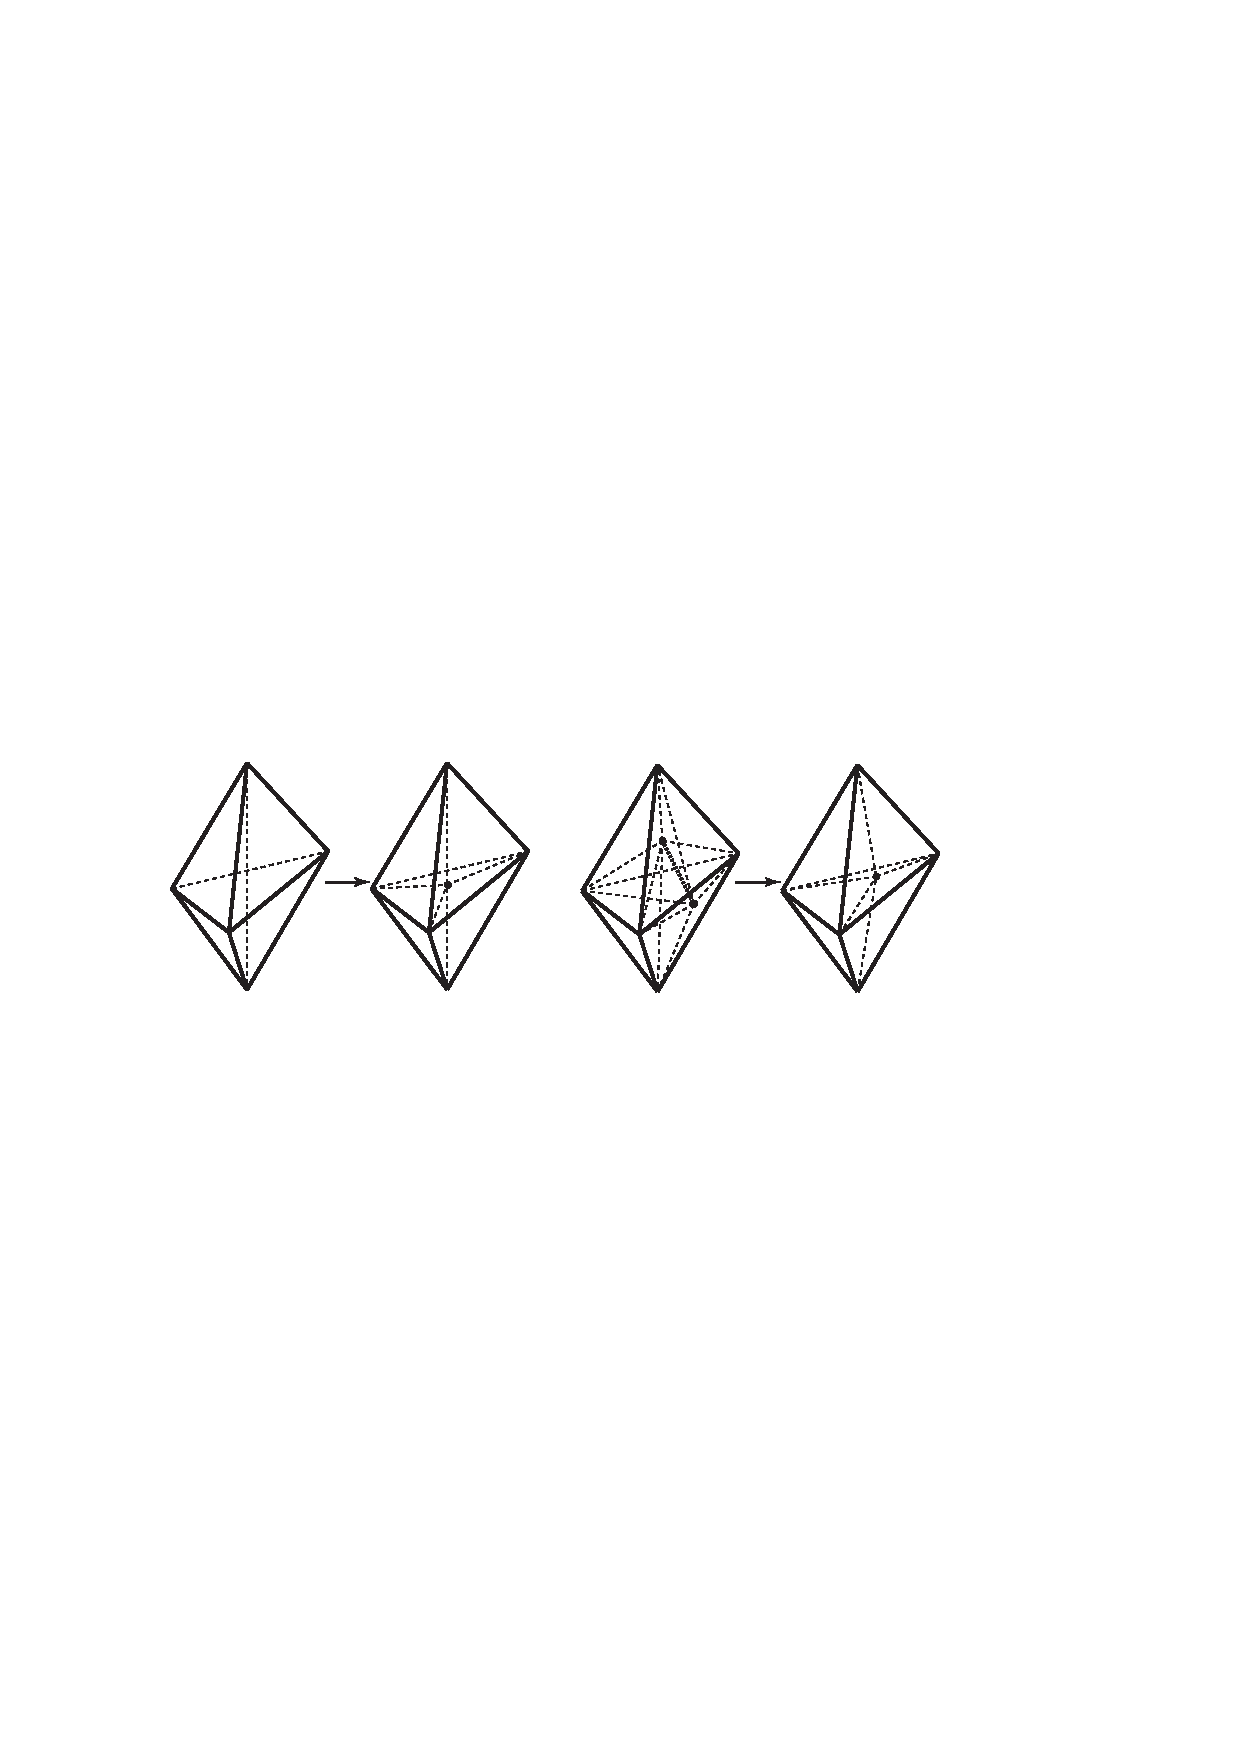
\includegraphics[width=8.0cm]{images/EdgeSplitCollapse}
\caption{Example of the edge split (left) and edge collapse (right)
  operations in 3D. The edge is split at its midpoint and the newly
  created node is then connected to the vertices of the elements
  containing the edge, thus creating additional elements. For edge
  collapse, the elements surrounding the edge are deleted and a node
  placed at the midpoint of the removed edge.}
\label{Fig:EdgeSplit}
\end{figure}
\begin{figure}
\centering
\noindent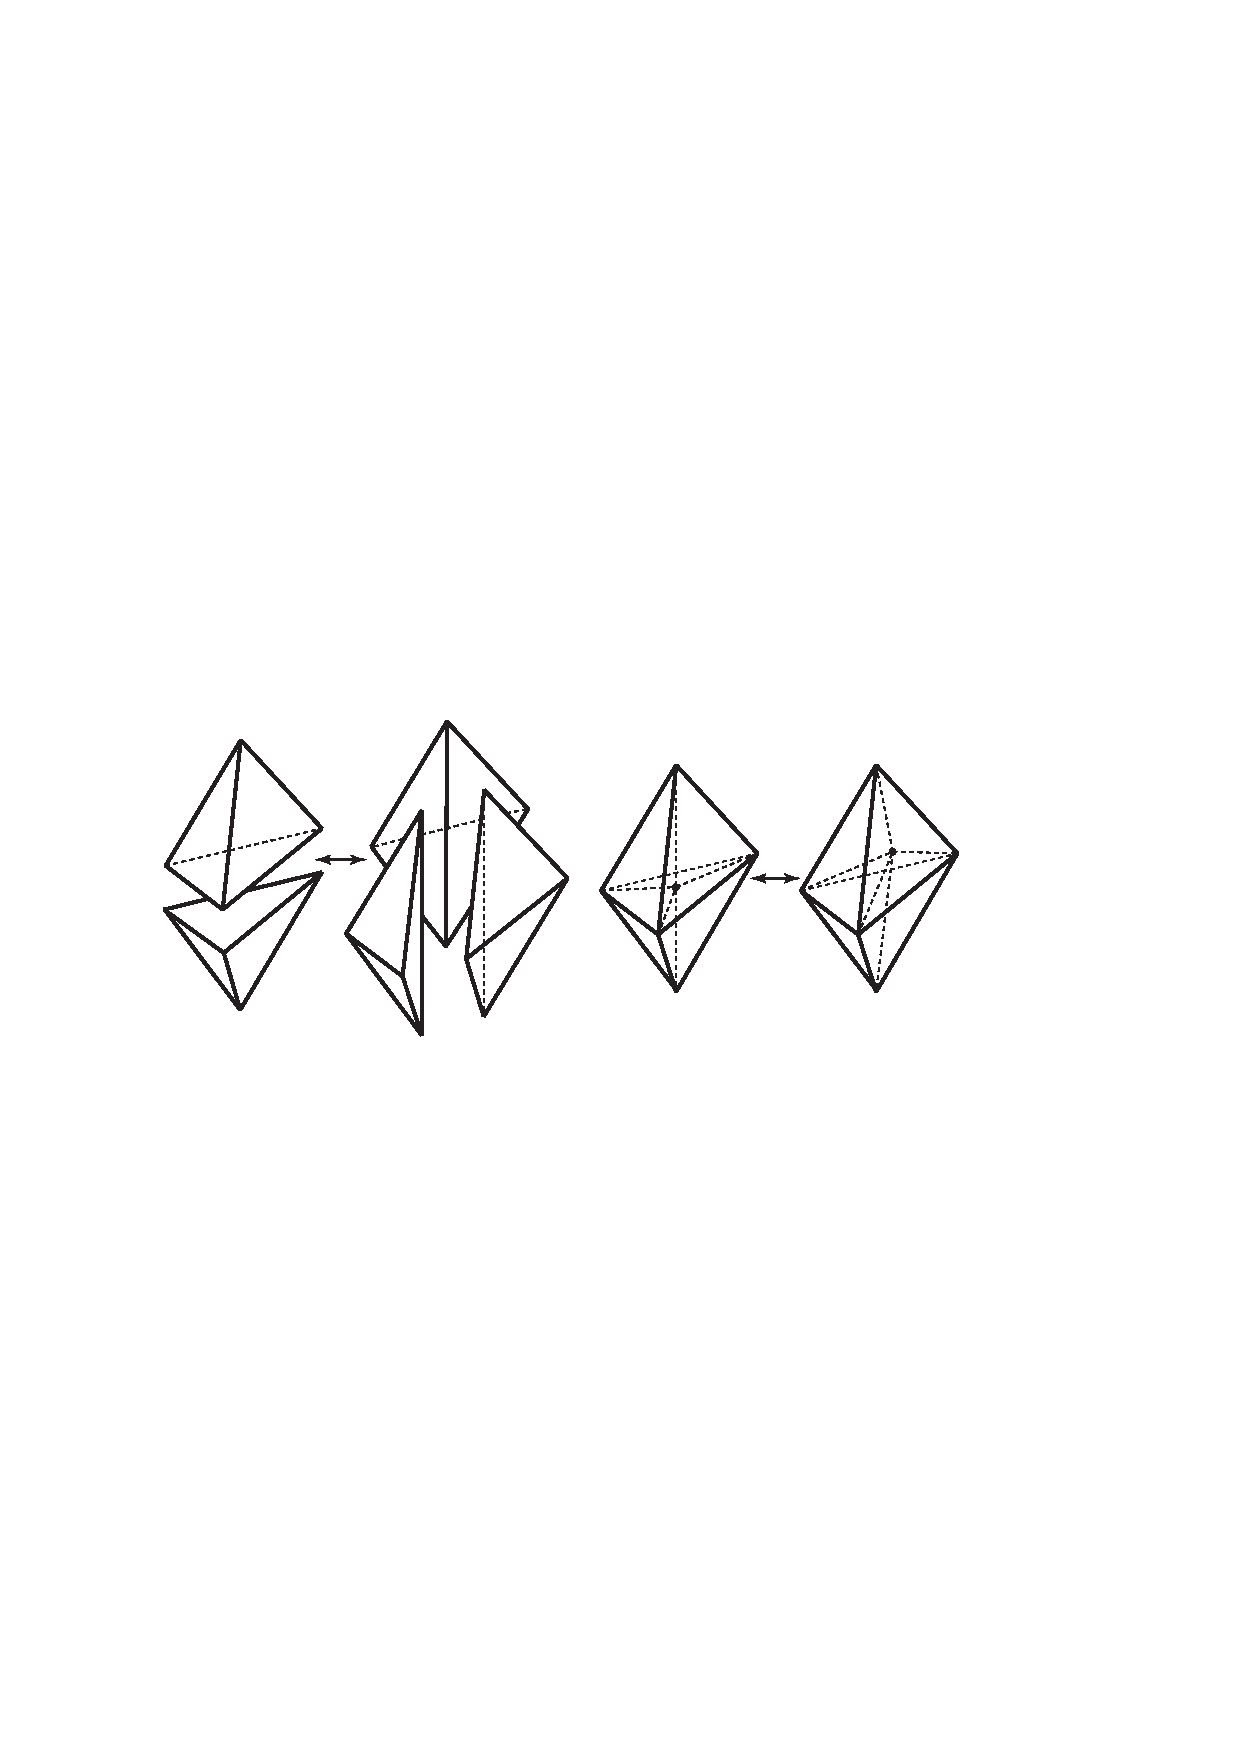
\includegraphics[width=8cm]{images/EdgeFaceNodeMove}
\caption{An example of the face to edge and edge to face swapping
  operation (left) and node movement (right) in 3D.}
\label{Fig:face2edge}
\end{figure}

\begin{figure}
\centering
\noindent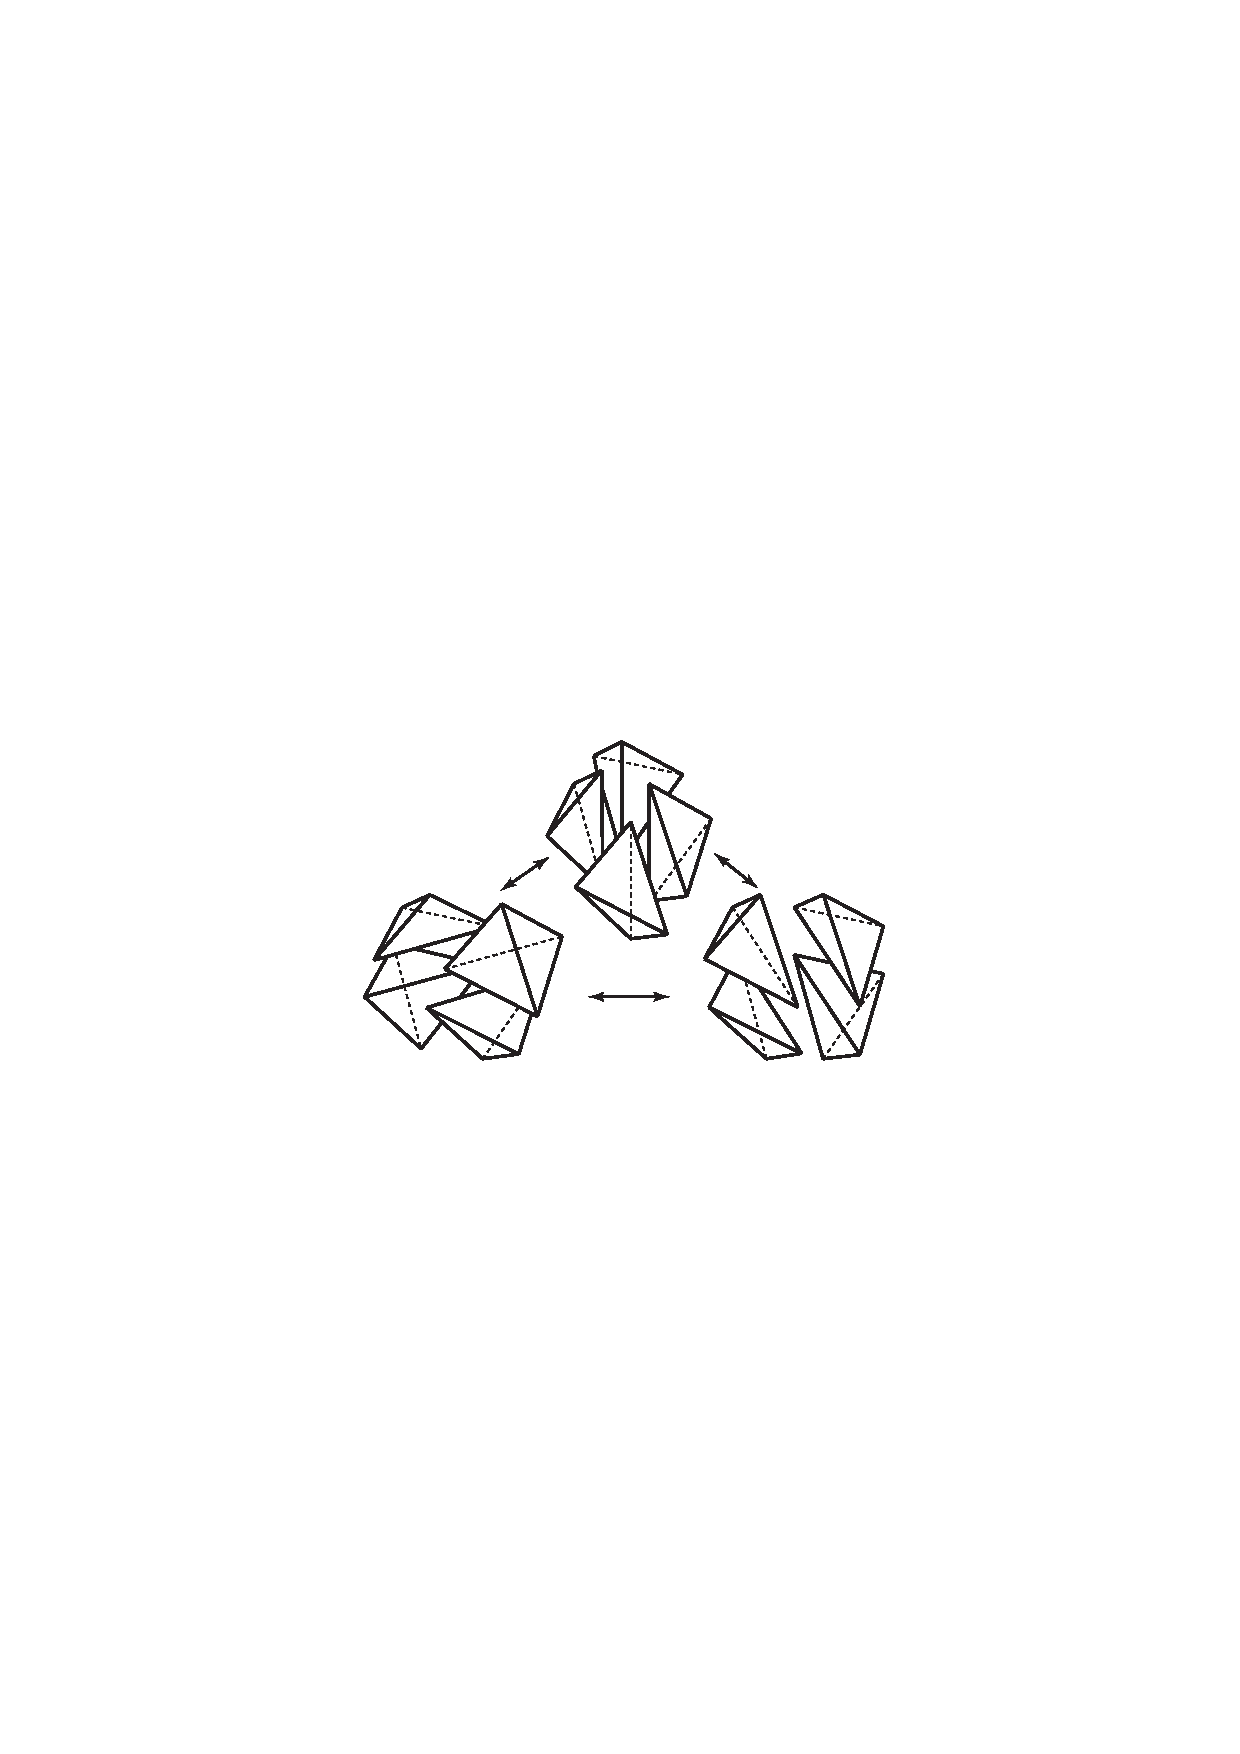
\includegraphics[width=7cm]{images/edge2edge}
\caption{An example of the topological operation of edge to edge
  swapping in 3D.}
\label{Fig:edge2edge}
\end{figure}

Approaches based on these operations are often referred to as mesh
optimisation methods since they involve the definition of some
objective function, usually a norm over the entire mesh of a local
mesh quality estimate. Optimisation of the mesh progresses by
improving the worst elements through a series of elemental
modifications to the mesh in an attempt to minimise the functional and
hence improve the overall quality of the mesh. Dynamic mesh
optimisation is achieved through the construction of metric with which
the objective functional is evaluated and which is itself dependent on
the computed solution fields \citep{simpson1994, buscaglia1997,
  pain2001, piggott2005, power2006}. This allows local anisotropic
features in a solution to be made isotropic in a warped domain through
a coordinate transformation.

\section{Mesh optimisation operations}

\begin{figure}
\centering
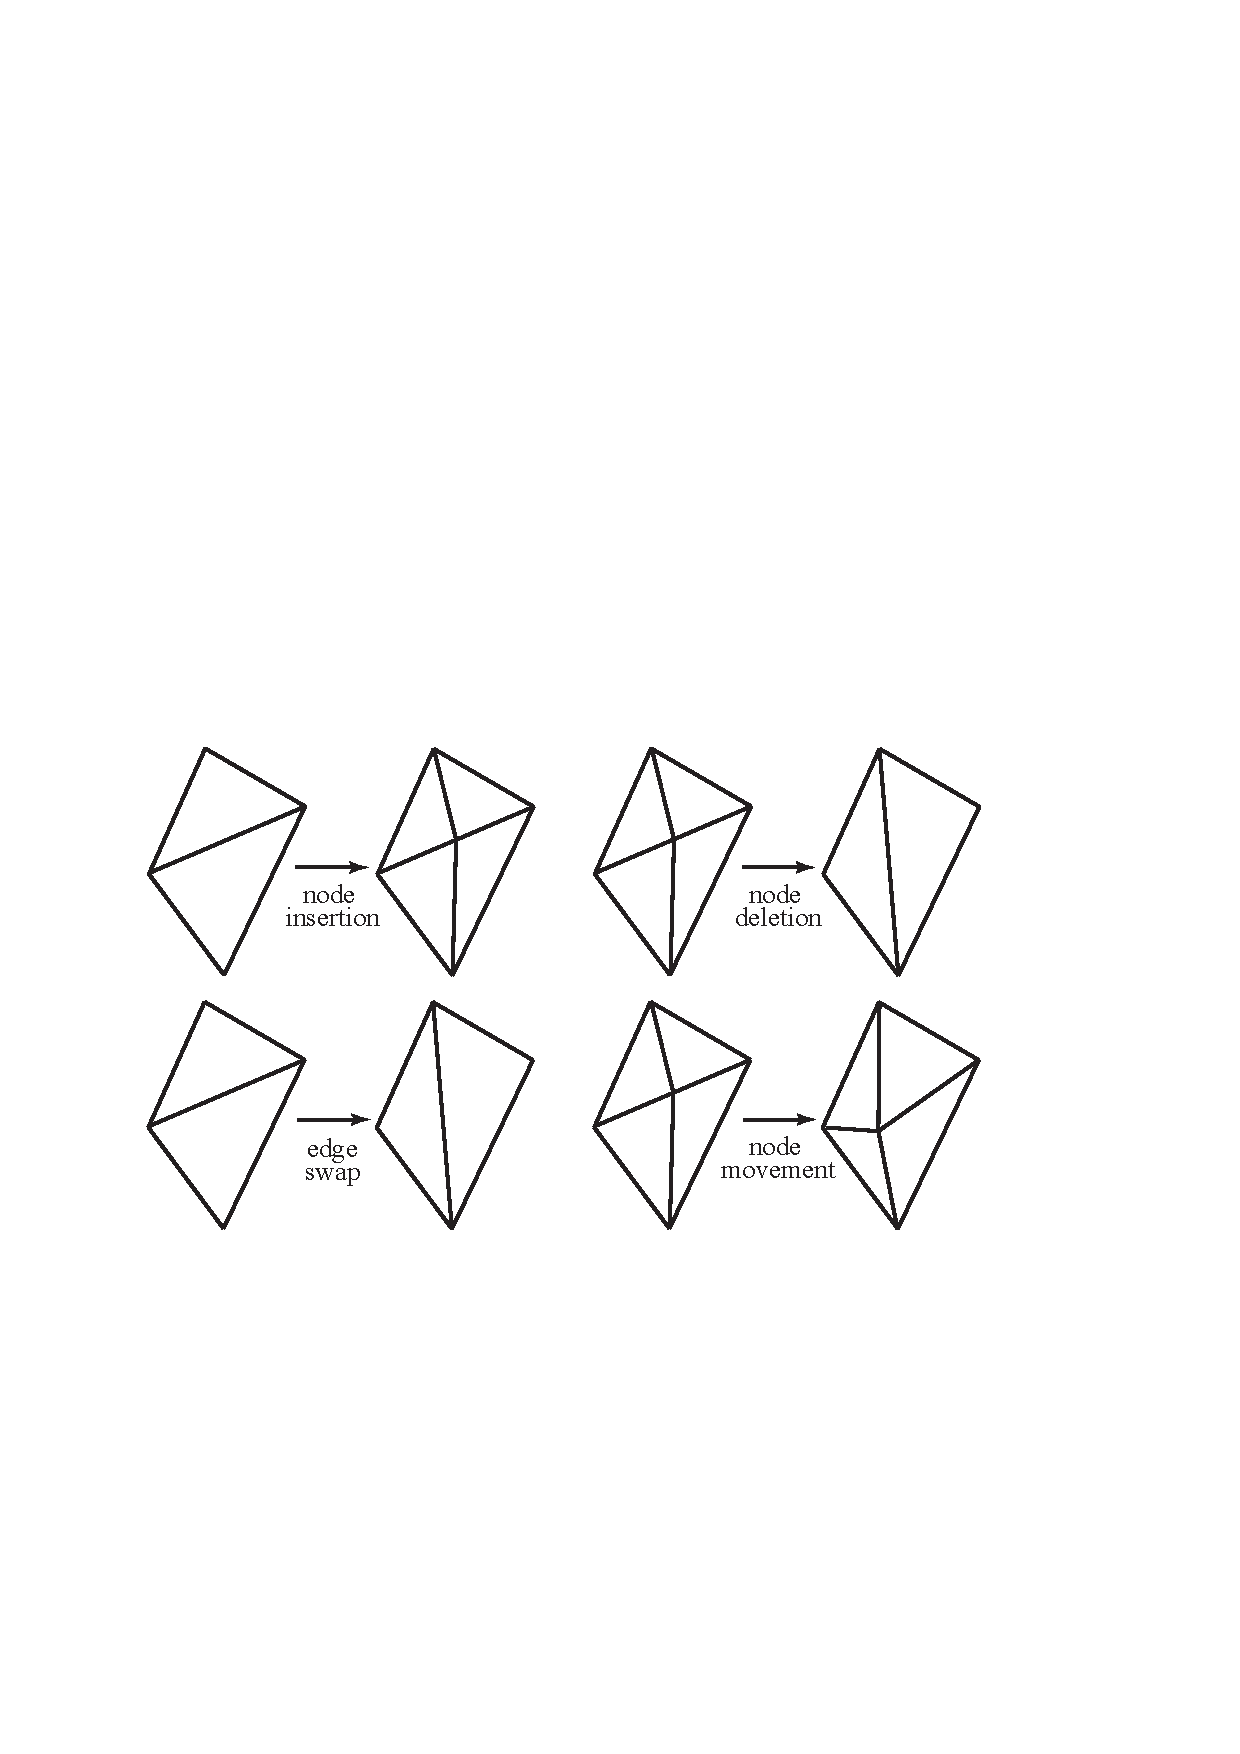
\includegraphics[width=10.0cm]{images/MeshOperations2D.pdf}
\caption{Local element operations used to optimise the mesh in two
  dimensions. Top-left: node insertion or edge split.  Top-right: node
  deletion or edge collapse. Bottom-left: edge swap. Bottom-right:
  node movement.}
\label{Fig:MeshOperations}
\end{figure}

Given an unstructured mesh and information regarding the ideal shape
and sizes of the elements making up the mesh, an optimisation-based
adaptivity algorithm can be formulated via the use of local
topological operations which seeks to improve the quality of elements.

In the examples presented in this work a two-dimensional mesh
optimisation algorithm \citep{agouzal1999,vasilevskii1999adaptive} is used
which employs the following local operations depicted in figure
\ref{Fig:MeshOperations}:
\begin{itemize}
\item Node insertion or edge split -- here a node is inserted on a
  pre-existing edge in the mesh so that the four new elements have
  improved shape/size characteristics than the original two; while the
  location of this new node along the pre-existing edge can be
  optimised, it is common to simply split it at its mid-point.
\item Node deletion or edge collapse -- here the inverse operation is
  performed where an edge in the mesh is collapsed, and consequently a
  node is deleted and two elements removed from the mesh.
\item Edge swap -- here an edge between two elements is removed and
  replaced with the only other possible configuration in two
  dimensions; the number of nodes and elements is preserved through
  the operation, but the edge lengths and elements shapes are
  manipulated.
\item Node movement -- here a node is moved so as to improve the
  quality of all the elements surrounding it; the direction in which
  to move the node can be calculated by considering a discrete
  gradient of the mesh quality functional and performing a line search
  in this direction.
\end{itemize}

The local operations employed in 3D are:
\begin{itemize}
\item{Edge split:} a node is inserted at the centre of an edge and
  surrounding elements created (Fig. \ref{Fig:EdgeSplit}).
\item{Edge collapse:} all elements belonging to the edge are deleted
  and the two nodes of the edge collapsed to its centre (Figure
  \ref{Fig:EdgeSplit}), in cases where one of the nodes is used to
  define the domain geometry the nodes are collapsed to that point, if
  both nodes define some geometrical structure then this operation is
  not permitted.
\item{Edge-face swap:} if two tetrahedra share a common face, and
  provided their combined interior is convex, the face is deleted and
  a new edge introduced between the two nodes not shared thus
  producing three tetrahedra with different alignment
  (Fig. \ref{Fig:face2edge}). The inverse operation where an edge is
  replaced by a face is also allowed.
\item{Edge-edge swap:} $S$ elements are assumed to lie around an edge
  which may be replaced by a different edge resulting in $2S-4$
  elements with different alignment (Fig. \ref{Fig:edge2edge}).
  \cite{freitag1997} found that for increasing $S$ the number of
  transformations that improve the mesh decline dramatically: for this
  reason, this operation is limited to $S\le 4$.
\item{Limited node movement:} the local topology of the mesh is
  preserved but mesh quality is improved by visiting each node and
  moving it to the centroid of all surrounding nodes, \ie\  ensuring
  that when measured in metric space the lengths of all edges attached
  to this node are approximately equal (Fig. \ref{Fig:face2edge}).
\end{itemize}

\section{The objective functional}
In order to decide whether the operations described above improve the
quality of the mesh, an objective functional measuring the quality of
the mesh must be defined.  The functional is constructed in order to
gauge mesh quality and whose maximisation is the goal of the
optimization algorithm.

Many measures of element quality have been proposed. In general, for
mesh generation applications Euclidean geometric metrics are
considered \cite{knupp2000achievingI,
  knupp2000achievingII}. However, these metrics do not take into
account characteristics of the solution. Therefore, other measures of
element quality have been proposed which do take into consideration both
the shape and size of the elements required for controlling solution
errors.

In the work described here, we use the element quality measure for 2D
simplexes proposed by Vasilevskii \etal\
\cite{vasilevskii1999adaptive}:
\begin{equation}\label{eqn:quality2D}
q^M(\triangle) = \underbrace{12\sqrt{3}\frac{|\triangle|_M}{|\partial\triangle|_M^2}}_{I} \underbrace{F\left(\frac{|\partial\triangle|_M}{3}\right)}_{II},
\end{equation}
where $|\triangle|_M$ is the area of element $\triangle$ and
$|\partial\triangle|_M$ is its perimeter as measured with respect to
the non-Euclidean metric $M$ as evaluated at the element's centre. The
first factor ($I$) is used to control the shape of element
$\triangle$. For an equilateral triangle with sides of length $l$,
$|\triangle| = l^2\sqrt{3}/4$ and $|\partial\triangle| = 3l$; and so
$I=1$. For non-equilateral triangles, $I<1$. The second factor ($II$)
controls the size of element $\triangle$. The function $F$ is smooth
and defined as:
\begin{equation}
F(x) = \left(\min(x, 1/x)(2 - \min(x, 1/x))\right)^3,
\end{equation}
which has a single maximum of
unity with $x=1$ and decreases smoothly away from this with
$F(0)=F(\infty)=0$. Therefore, $II=1$ when the sum of the lengths of the
edges of $\triangle$ is equal to $3$, \eg\ an equilateral triangle with
sides of unit length, and $II<1$ otherwise. Hence, taken together, the
two factors making up $Q$ yield a maximum value of unity for an
equilateral triangle with edges of unit length, and $Q$ is less than
one otherwise. 

We use an analogous measure of element quality proposed by Agouzal
\etal\ for 3D simplexes \cite{agouzal1999}.

Mesh optimization is now performed on the mesh via a sequence of local
topological and geometrical operations \citep{pain2001,freitag1997}
which seek to efficiently minimise the objective functional. The algorithm
proceeds in a Gauss-Seidel iterative manner. Each of the elements are
visited in turn and the local mesh structure of the element and its
neighbours altered via the operations described above. If an operation
is found to improve the mesh quality as measured by the functional,
it is retained.

%\chapter*{\pragmatic\ Primer}
% \pagenumbering{roman} \setcounter{page}{}

Please check the \pragmatic\ webpage at
\href{https://launchpad.net/pragmatic}{https://launchpad.net/pragmatic}
to ensure you are reading the most recent version of this
manual. Methods for installing \pragmatic\ may sometimes change, and
instructions may be updated!

This is a one-page primer for obtaining \pragmatic\ and getting up and
running with development. It assumes that:

\begin{itemize}
\item You are running Ubuntu Linux, release 11.10 or newer
\item You have administrative rights on your computer
\item You know how to run a terminal with a command prompt
\item You have a directory in which you can create files
\end{itemize}

Set up your computer to access the \pragmatic\ repository by typing:

\begin{lstlisting}[language=Bash]
sudo apt-add-repository -y ppa:pragmatic-core/ppa
\end{lstlisting}

Type your password when prompted.

Once this completes, update your system and install \pragmatic along with its
supporting software by typing:

\begin{lstlisting}[language=Bash]
sudo apt-get update
sudo apt-get -y install pragmatic
\end{lstlisting}

To get dOxygen documentation of the API point your browser at:
\begin{lstlisting}[language=Html]
fiel:///usr/share/pragmatic/html/index.html
\end{lstlisting}


\makeatletter
\renewcommand\l@section{\@dottedtocline{1}{1.5em}{2.7em}}
\renewcommand\l@subsection{\@dottedtocline{2}{4.2em}{3.6em}}
\renewcommand\l@subsubsection{\@dottedtocline{3}{7.8em}{4.5em}}

% new command to add Word-style comments to text
\newsavebox{\marginbox}% contains the contents of the comment environment
\let\comment\relax% removes and previous definition of \begin{comment}
\let\endcomment\relax% removes any previous definition of \end{comment}
\newenvironment{comment}{
  \begin{lrbox}{\marginbox}
  \begin{minipage}{\marginparwidth}
  \footnotesize
  }{
  \end{minipage}
  \end{lrbox}
  \marginpar{\usebox{\marginbox}}
  }

\makeatother

{ \setlength{\parskip}{0pt} \tableofcontents \listoffigures }

\newpage \clearpage \thispagestyle{plain}

\mainmatter

%\include{getting_started}
%\include{model_equations}

% Whole bunch of format hacking because Bibliography isn't a real chapter.
\cleardoublepage
\phantomsection
\renewcommand\leftmark{}
\renewcommand\rightmark{Bibliography}
\addcontentsline{toc}{chapter}{Bibliography}
\bibliography{bibliography}

\appendix

%\include{about}

\cleardoublepage
\phantomsection
\renewcommand\leftmark{}
\renewcommand\rightmark{Index}
\addcontentsline{toc}{chapter}{Index}
\printindex

\end{document}
